\documentclass [pdftex,12pt] {report}
\usepackage [utf8x]{inputenc}
\usepackage [french] {babel}
\usepackage[pdftex]{graphicx}
\usepackage{sidecap}
\usepackage{float}
\usepackage{natbib,hyperref}
\usepackage{indentfirst}
\usepackage[T1]{fontenc} 
\usepackage{amsfonts}
\usepackage{tabularx}
\usepackage{listings}
\usepackage{color}
\usepackage{xcolor}
\usepackage{caption}
\usepackage{textcomp}
\usepackage{adjustbox}

\usepackage{titlesec}
\titleformat{\chapter}[hang]{\Huge\bfseries}{\thechapter\hsp\textcolor{gray75}{|}\hsp}{0pt}{\Huge\bfseries}
\titlespacing*{\chapter}{0pt}{-40pt}{40pt}

\usepackage{hyperref}
\hypersetup{
  backref=true,
  pagebackref=true,
  hyperindex=true,
  breaklinks=true,
  colorlinks=true,
  urlcolor=blue,
  linkcolor=black,
  citecolor=black
}
\definecolor{gray75}{gray}{0.75}
\definecolor{gray}{rgb}{0.4,0.4,0.4}
\definecolor{darkblue}{rgb}{0.0,0.0,0.6}
\definecolor{lightblue}{rgb}{0.0,0.4,0.9}
\definecolor{cyan}{rgb}{0.0,0.6,0.6}
\definecolor{dkgreen}{rgb}{0,0.6,0}
\definecolor{gray}{rgb}{0.5,0.5,0.5}
\definecolor{mauve}{rgb}{0.58,0,0.82}
\definecolor{forestgreen}{RGB}{34,139,34}
\definecolor{orangered}{RGB}{239,134,64}
 
\lstdefinestyle{Java}{
  language=Java,
  basicstyle=\footnotesize\ttfamily,
  numbers=left,
  numberstyle=\tiny\color{gray},
  stepnumber=1,
  numbersep=5pt,
  backgroundcolor=\color{white},
  showspaces=false,
  showstringspaces=false,
  showtabs=false,
  frame=single,
  rulecolor=\color{black},
  tabsize=4,
  breaklines=true,
  breakatwhitespace=false,
  title=\lstname,
  keywordstyle=\color{lightblue},
  commentstyle=\color{dkgreen},
  stringstyle=\color{mauve},
  escapeinside={\%*}{*)},
  keywords=[2]{DATA},
  keywordstyle=[2]\color{red},
  morekeywords={R,View,ViewGroup,TextView,ImageView,ViewHolder}
}

\lstdefinestyle{XML} {
    language=XML,
    frame=single, 
    extendedchars=true, 
    breaklines=true,
    breakatwhitespace=true,
    emph={},
    emphstyle=\color{red},
    basicstyle=\small\ttfamily,
    columns=fullflexible,
    commentstyle=\color{gray}\upshape,
    morestring=[b]",
    morecomment=[s]{<?}{?>},
    morecomment=[s][\color{forestgreen}]{<!--}{-->},
    keywordstyle=\color{orangered},
    stringstyle=\ttfamily\color{black}\normalfont,
    tagstyle=\color{darkblue}\bf,
    morekeywords={attribute,xmlns,version,type,release},
}


\lstdefinestyle{HTML} {
    language=HTML,
    frame=single, 
    extendedchars=true,
    showspaces=false,
    showstringspaces=false,
    showtabs=false,
    breaklines=true,
    breakatwhitespace=true,
    emph={},
    emphstyle=\color{darkblue},
    basicstyle=\tiny\ttfamily,
    columns=fullflexible,
    commentstyle=\color{gray}\upshape,
    morestring=[b]",
    morecomment=[s]{<?}{?>},
    morecomment=[s][\color{dkgreen}]{<!--}{-->},
    keywordstyle=\color{purple},
    stringstyle=\ttfamily\color{black}\normalfont,
    tagstyle=\color{lightblue}\bf,
}

\lstset{language=Java,frame=lines}
\lstset{language=XML,frame=lines}


\def\wl{\par \vspace{\baselineskip}}
\renewcommand{\lstlistingname}{Code}
\newcommand{\HRule}{\rule{\linewidth}{0.5mm}}
\newcommand{\hsp}{\hspace{20pt}}

\begin {document}

\begin{titlepage}
\begin{center}

% Upper part of the page. The '~' is needed because \\
% only works if a paragraph has started.

\includegraphics[width=0.15\textwidth]{./resources/ub.png}~\\[1cm]

\textsc{\LARGE Université de Bordeaux}\\[1.5cm]

\textsc{\Large {Architecture Logicielle Distribuée et Adaptative}}\\[0.5cm]

% Title
\HRule \\[0.4cm]
{ \huge \bfseries Freya Web Application}\\[0.4cm]

\HRule \\[1.5cm]

% Authors, clients and supervisor
\begin{minipage}{0.4\textwidth}
\begin{flushleft} \large
\emph{Auteurs:} \\
Elyas \textsc{Ben Hadj Yahia}\\
Rémi \textsc{Delassus}\\
David \textsc{Frenandez}\\
Ryan \textsc{Herbert}
\end{flushleft}
\end{minipage}
\begin{minipage}{0.4\textwidth}
\begin{flushright} \large
\emph{Enseignant:} \\
David \textsc{Bromberg}\\
\end{flushright}
\end{minipage}

\vfill

% Bottom of the page
{\large \today}

\end{center}
\end{titlepage}


\tableofcontents
\newpage 

\chapter{Présentation}
Freya est une application web conçue pour faciliter la gestion des musées aux
conservateurs.\\
Ce projet a été mis en place grâce à de nombreux outils et frameworks, notamment
Maven\footnote{Maven: \url{http://maven.apache.org/}} et Google App
Engine\footnote{Google App Engine:
\url{https://developers.google.com/appengine/}}.\\
Le dépôt de code source du projet Freya se situe à cette
adresse\footnote{freya: \url{https://github.com/elyas-bhy/freya}}.


\section{Maven}
Maven est un outil de gestion de projet. Il permet notamment de spécifier
comment un logiciel doit être compilé, et décrire ses dépendances. Il permet
aussi d’intégrer des plugins dans des phases de compilation spécifiques, ce qui
permet d’avoir un environnement configurable.

\section{Google App Engine}
Google App Engine (GAE) est une PaaS (Platform as a Service) qui fournit un
ensemble d’outils afin de faciliter le développement d’applications web. Cette
plateforme met à disposition du développeur un runtime Java, une base de données
NoSQL (appellée \emph{datastore}), et l’hébergement de l’application web sur les
serveurs Google.\\

Afin d’intéragir avec le datastore, on peut utiliser plusieurs méthodes
différentes, comme par exemple l’API Datastore de bas niveau, JPA, JDO, ou
encore d’autres bibliothèques tierces comme Objectify.
Freya a été conçu en utilisant l’implémentation JPA 2.0 de
DataNucleus\footnote{DataNucleus:
\url{https://code.google.com/p/datanucleus-appengine/}} pour sa compatibilité avec GAE.\\

GAE fournit aussi une console d’administration très complète pour monitorer
l’état de l’application web, le traffic, les requêtes, les logs, etc...

\chapter{Architecture du backend}

\section{Entités}
\begin{figure}[h]
  \center
  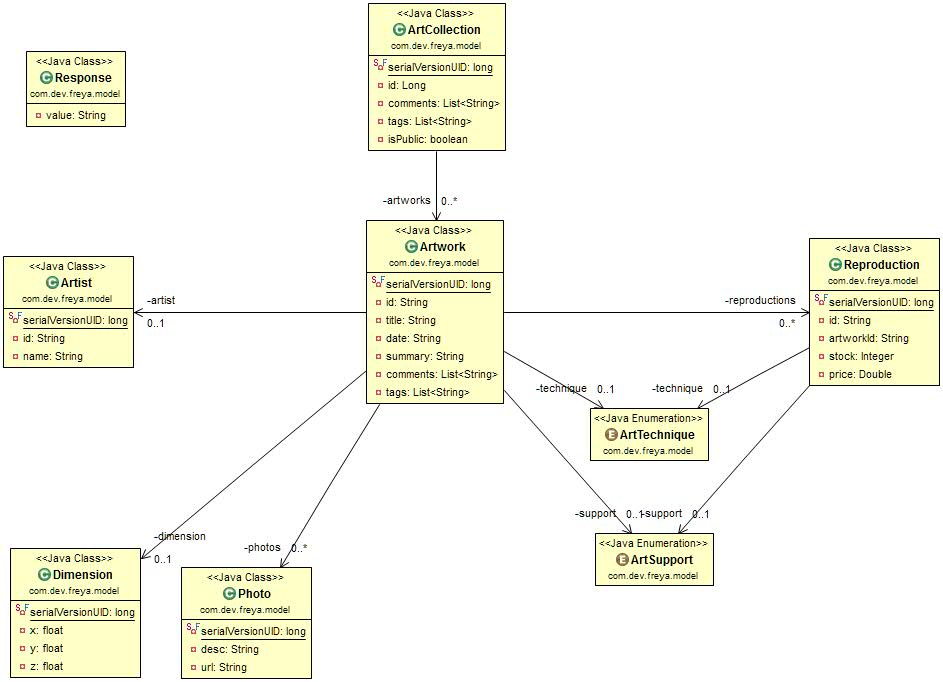
\includegraphics[width=1.0\textwidth]{resources/model_diagram.jpg}
  \caption{Diagramme de classe des entités}
  \label{fig:model_diagram}
\end{figure}

\newpage
\section{Conception}
Une des difficultés majeures de ce projet a été de concevoir correctement les
relations entre les entités afin d’être en accord avec les restrictions de GAE.
Étant donné que le \emph{datastore} est une base de données NoSQL, il fallait
respecter plusieurs contraintes supplémentaires.\\

Une des contraintes est qu’il faut qu’une entité fille encode la clé de son
parent dans sa propre clé. Cela signifie que quand une entité fille est
persistée, son parent ne peut plus changer (c.à.d être remplacé par un autre
parent). Ceci est dû au fait que les entités fille et parent sont placées dans
le même \emph{entity group}, et qu’une entité ne peut appartenir qu’à un seul
\emph{entity group}.\\

Pour des raisons de performance, le \emph{datastore} met en place d’autres
restrictions au niveau des requêtes. En effet, certaines opérations ne sont pas permises
(subqueries, fonction size, joins complexes, opérateur MEMBER OF sur une
collection non-primitive, et d'autres).\\

Pour gérer les paramètres optionnels pour filtrer les recherches, nous avons
utilisé l’API Criteria\footnote{JPA Criteria API:
\url{http://www.objectdb.com/java/jpa/query/criteria}} de JPA afin d’avoir un
code propre et maintenable, et qui est beaucoup plus robuste comparé à la
création de la requête par concaténation de chaînes.\\

Afin d'améliorer les performances du backend, nous avons aussi mis en place
Memcache\footnote{Memcache:
\url{https://developers.google.com/appengine/docs/java/memcache/}}, un système
de cache afin d'accélérer les requêtes d'écriture.

\chapter{API REST}

L’un des avantages de GAE est qu’il permet de facilement mettre en place une API
REST et de l’exposer, grâce au module Google Cloud Endpoints
(GCE)\footnote{GCE:
\url{https://developers.google.com/appengine/docs/java/endpoints/}}.

Pour ce faire, on a simplement à annoter une classe comme étant une API, et
déclarer les méthodes d’API (notamment routes, paramètres, méthodes HTTP).\\

\begin{adjustbox}{minipage=1.02\textwidth,margin=0pt \smallskipamount,center}
\begin{lstlisting}[style=Java, label=endpoints, caption=Exemple d'API avec
Google Cloud Endpoints]
@Api(name = "myapi", version = "v1")
public class MyEndpoints {

	@ApiMethod(
	    name = "elements.get",
	    path = "elements/{element_id}",
	    httpMethod = HttpMethod.GET
	)
	public Element getElement(@Named("element_id") String id) {
	    // ...
	}
}
\end{lstlisting}
\end{adjustbox}


GCE se chargera ensuite de construire et déployer l’API avec la description des
méthodes exposées.\\
La description de l’API Freya (v1) se situe à cette
adresse\footnote{Descriptif:
\url{https://github.com/elyas-bhy/freya/wiki/freya-RESTful-API}}.\\
La version déployée de cette API se situe à cette adresse\footnote{Version
déployée de l'API: \url{http://goo.gl/o9GGBB}}.\\

Exemple d’interaction avec l’API en utilisant curl:
\begin{verbatim}
curl --header “Content-Type: application/json” -X GET
https://freya-app.appspot.com/_ah/api/freya/v1/artworks
\end{verbatim}

\chapter{Bibliothèque client}

Un autre avantage de GCE est qu’il permet de générer automatiquement des
bibliothèques clients multi-plateformes (Java/Android, iOS, JavaScript) afin de
faciliter l’interaction avec l’API.
La bibliothèque client consiste en deux parties différentes:\\

\textbf{Le modèle client}: représentation en Java des entités manipulables. Ces
classes représentent le modèle existant du backend. Elles étendent la classe GenericJson
afin d’être sérialisable sur le réseau.
Exemple: le client dispose de la classe Artist (et son agrégat
ArtistCollection\footnote{Des classes de type agrégats sont générés aussi car on
peut sérialiser que des objets de type “bean”, c.à.d avec des getters/setters.
Les objets de type List<Object> ne sont pas conformes et doivent donc être
encapsulés dans une classe ObjectCollection.}), générée par GCE. Cette classe
est une représentation fidèle à celle du backend.\\

\textbf{Builders et stubs}: servent à faciliter la communication avec le
backend.
La classe générée Freya (nom de l’application) met en place une interface facile
à utitliser pour le client afin d’exécuter des méthodes de l’API.\\


\begin{adjustbox}{minipage=0.92\textwidth,margin=0pt \smallskipamount,center}
\begin{lstlisting}[style=Java, label=endpoints, caption=Exemple d'utilisation
de la bibliothèque client]
Artwork a = freya.artworks().get(artworkID).execute();
\end{lstlisting}
\end{adjustbox}
\chapter{Front-end}

Pour mettre en place le front-end de Freya\footnote{Front-end Freya:
\url{http://freya-app.appspot.com/}}, nous avons voulu profiter de la
bibliothèque client générée pour pouvoir accéder à l’API directement, sans
passer par des étapes intermédiaires. C’est la raison pour laquelle nous avons
choisi d’utiliser des pages JSP plutôt qu’utiliser GWT, qui est assez lourd à
mettre en place et très verbeux.

\section{Site web}

Le front-end de notre projet est un site Internet constitué de pages JSP. Ce
site est organisé de la manière suivante:\\

- A la racine du site (\emph{webapp}), un fichier \emph{index.jsp} sert de point
d’entrée par défaut dans l’application.\\

- Un dossier \emph{includes} regroupe les pages qui ne sont pas destinées à être
affichées seules mais qui sont là pour factoriser du code, notamment les parties
statiques du site (header, footer), mais aussi les manières de lister des
éléments.\\

- Pour chaque entité, un dossier contenant les fichiers \emph{view.jsp},
\emph{edit.jsp} et \emph{list.jsp} qui leurs sont propres. Le fichier
\emph{view} permet d’accéder à la vue détaillée d’une entité, permettant de
consulter l’ensemble de ses champs. Le fichier \emph{edit} permet de créer et
modifier une entité en renseignant ses champs. Le fichier \emph{list} permet de
lister l’ensemble des entités d’un même type. Pour cela il utilise le fichier à
inclure sachant lister une sous-partie ou l’ensemble de ces entités.

\newpage
\section{JavaScript}


Nous avons eu recours à plusieurs bibliothèques JavaScript, notamment JQuery et
ses modules DataTables, Chosen et Tabs.
Nous avons choisi ces plugins afin de rendre l’interface plus agréable à
utiliser.\\

Le plugin DataTables nous permet d’ajouter beaucoup de fonctionnalités à nos
tableaux. Notamment la pagination des données, et la possibilité de trier le
tableau suivant les colonnes.
De plus, DataTables peut être appliqué sur un tableau HTML existant, ou
encore nous pouvons lui passer en entrée des données en JSON, et lui demander de
construire la table lui-même.\\

Chosen est un plugin qui s’applique aux menus déroulants, permettant d’effectuer
des recherches au sein des menus, tout en appliquant une modification esthétique
agréable.\\

Le plugin Tabs est un outil de tabulation de div. Avec ce plugin nous avons pu
rendre plus agréable la disposition des pages présentant plusieurs tables. Avec
ce plugin, nous pouvons également spécifier, à l’aide d’un suffixe à l’URL, la
tabulation à afficher en priorité au moment du chargement de la page.

\chapter{Difficultés}

La mise en place de ce projet n'a pas été sans contraintes:\\

\begin{itemize}
\item Maven: conflits entre versions des dépendances
\item Restrictions GAE et comportements inattendus
\item Contraintes NoSQL
\item Prise en main de l'API Criteria
\item Mise en place et maintien du cache (backend)
\item Développement du front-end
\end{itemize}

\end{document}
 
